\chapter{Glavna ploča}
\label{pog:mainboard}

Sustav se sastoji od dva uređaja koji rade u simbiozi. Glavna ploča služi za snimanje, obradu i pohranu glasovnih podataka i obradu i pohranu biomedicinskih parametara. Za snimanje biomedicinskih parametara koristi se narukvica. U ovom poglavlju se opisuje glavna ploča.

Zahtjevi na glavnu ploču su sljedeći:
\begin{itemize}
    \item mikrokontroler \engl{Microcontroler Unit, MCU}, dovoljno moćan za pokretanje neuralnih mreža i obradu podataka
    \item konektor za SD karticu
    \item bežična komunikacija putem Wi-Fi ili Bluetooth sučelja
    \item praćenje vremena putem RTC-a
    \item mikrofon za prikupljanje govora korisnika
    \item sučelja za testiranje i prženje koda na mikrokontroler
    \item napajanje i punjenje baterije preko USB C priključka
    \item baterijsko napajanje putem litij-ionske baterije
\end{itemize}
U daljnjem tekstu ovog poglavlja opisane su odabrane komponente, kao i razlog njihova odabira, način, razlozi i proračuni dizajna pojedinih podsustava, te dizajn, proizvodnja i testiranje PCB-a.

\section{Mikrokontroler}
Za mikrokontroler odabran je STM32F746VG baziran na Cortex-M7 arhitekturi koji integrira funkcionalnosti digitalne obrade signala, bogat sa svim potrebnim periferijama za integriranje s ostatkom sustava i dovoljno procesorske snage za obavljanje zadanog zadatka. Također, programska potpora je razvijena na razvojnom sustavu BLABLABLA, pa je ovaj mikrokontroler odabran radi lakšeg razvoja cjelokupnog sustava. Shema napajanja mikrokontrolera prikazana je na slici \ref{slk:MCU_PS}, a shema spajanja mikronotrolera sa ostatkom sustava prikazana je na slici \ref{slk:MCU_PE}.

\begin{figure}[hbt]
    \centering
    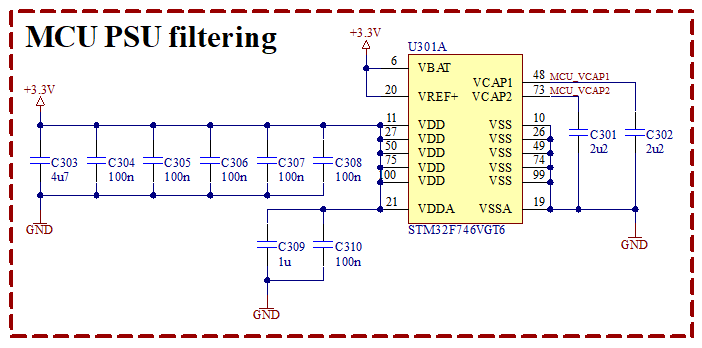
\includegraphics[width=\textwidth]{Figures/MCU_02.png}
    \caption{Shema napajanja mikrokontrolera}
    \label{slk:MCU_PS}
\end{figure}

Shema napajanja napravljena je prema uputama proizvođača \cite{stmicroelectronics:an4661}. S obzirom na to da na ovoj ploči nema analognih signala, nije potrebno raditi analogno-digitalnu pretvorbu, pa su stezaljke za napajanje analognog dijela mikrokontrolera spojene sa stezaljkama za napajanje digitalnog dijela. Također, nije potrebna precizna naponska referenca, a baterijskim napajanjem će upravljati vanjski čip, pa su te dvije stezaljke spojene na napajanje od +3.3V.

\begin{figure}[hbt]
    \centering
    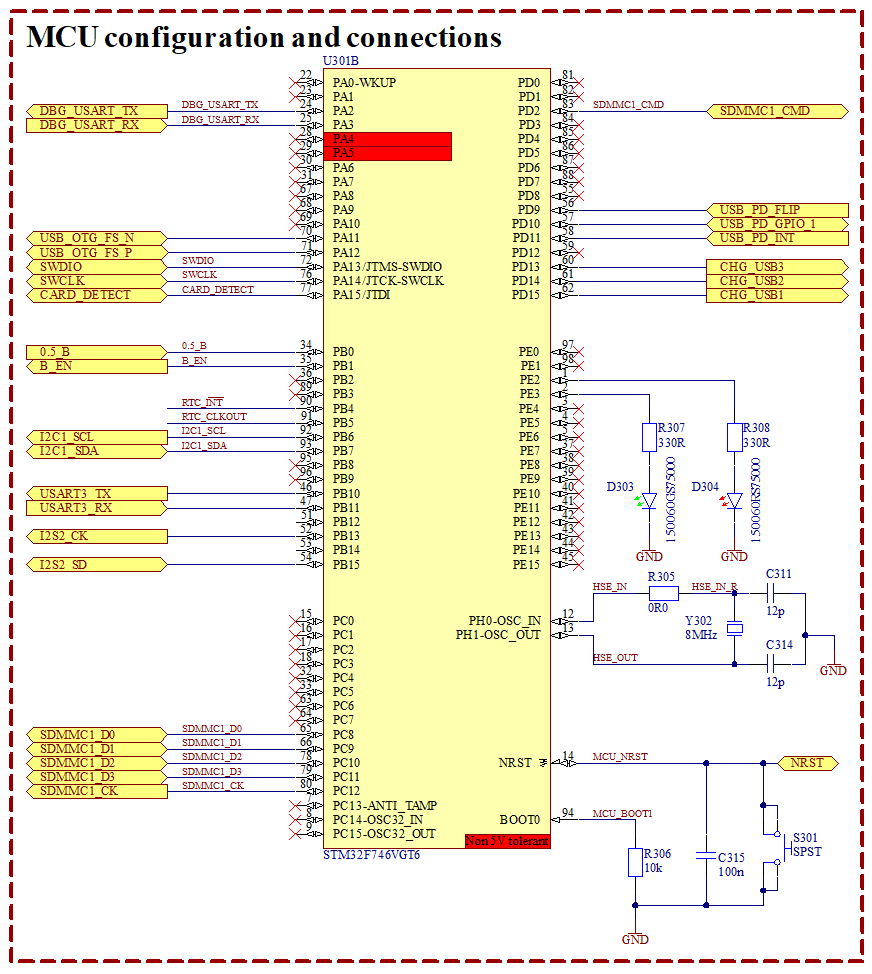
\includegraphics[width=\textwidth]{Figures/MCU_01.png}
    \caption{Shema periferije mikrokontrolera}
    \label{slk:MCU_PE}
\end{figure}

Prilikom dizajna 